\chapter{Accretion Disc Winds}
\label{sec:winds}

\epigraph{``A view of space, with an elephant obstructing it"}
{{\sl Mike Vennart, Silent/Transparent}}


%%%%WINDS 
%%% COULD MAKE THIS A NEW CHAPTER
\section{Observational Evidence}

The observational evidence for mass-loaded outflows or winds is 
widespread across the entire astrophysical mass range and most of
the electromagnetic spectrum. Before detailing the more compelling aspects
of this evidence, it is pertinent to briefly discuss the `smoking gun'
used to unambiguously detect winds -- the presence of blue shifted BALs
or `P-Cygni' profiles in an objects spectrum. 

Figure~?? shows how a spherical outflow of significant opacity will 
cause these characteristic line profile shapes to form, as scattering out of the line of sight 
causes a dip in the blue wing of the line, while scattering into the 
line of sight from other portions of the outflow causes an increase in flux
in the red wing of the line. The situation is much more complex in most
astrophysical situations; for example, the geometry is rarely spherically 
symmetric, and the line is rarely a pure scattering case. Indeed, the potential 
for complicated radiative transfer effects and variety in line formation mechanisms
is one of the reasons why 3D Monte Carlo radiative transfer simulations are necessary
to effectively model disc winds (see section 3).

\subsection{Cataclysmic Variables}

It has been known for a long time that winds emanating from the
accretion disc are important in shaping the ultraviolet (UV) spectra
of high-state CVs \citep{heap1978, greensteinoke1982}. The most spectacular evidence for such
outflows are the P-Cygni-like profiles seen in UV resonance lines such as
\civfull\ \citep[][; see figure~\ref{fig:cordova}]{cordova1982}). 
Considerable effort has been spent over the
years on understanding and modelling these UV features 
\citep[e.g.][]{drewverbunt1985,maucheraymond1987,SV93,KWD96,
kd1997,knigge1997,LK02,noebauer,puebla2011}. 
The basic picture emerging from these efforts is
of a slowly accelerating, moderately collimated bipolar
outflow that carries away $\simeq 1\% - 10\%$ of the accreting
material. State-of-the-art simulations of line formation in this type
of disc wind can produce UV line profiles that are remarkably similar
to observations, as shown in figure~\ref{fig:zcam_lk02}.

\begin{figure}
\centering
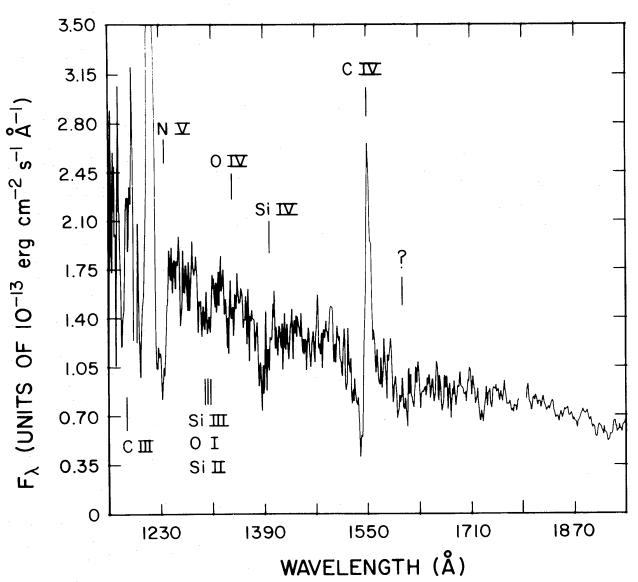
\includegraphics[width=0.8\textwidth]{figures/02-outflows/cordova_mason.png}
\caption
{
{\sl Credit: Cordova \& Mason 1982}. 
UV spectrum of the DN TW Vir during outburst. The P-Cygni profiles
can be seen clearly, demonstrating that a strong, fast outflow is present
in the system. 
} 
\label{fig:cordova}
\end{figure}

\begin{figure}
\centering
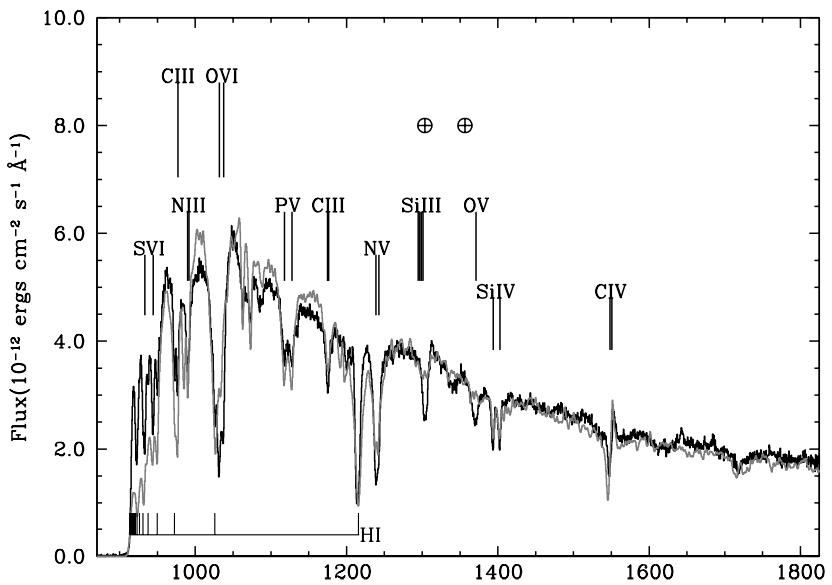
\includegraphics[width=0.8\textwidth]{figures/02-outflows/zcam_lk02.png}
\caption
{
{\sl Credit: Long \& Knigge 2002}. 
UV spectrum of Z Cam, compared to a synthetic spectrum from MCRT simulations.
} 
\label{fig:zcam_lk02}
\end{figure}

Much less is known about the effect of these outflows on the optical
spectra of high-state CVs. Direct evidence of wind-formed lines comes from
isolated observations of P-Cygni-like line profiles in
\ha\ and He \textsc{i} $\lambda5876$, \citep{patterson1996, RN98, kafka2004}. 
However, the effect on
the {\em emission} aspects of the optical spectrum is not well known.
\cite{MC96, MC97} have shown that the presence of disc winds may
offer a natural explanation for the single-peaked optical emission lines in
high-state CVs, since they can strongly affect the radiative transfer
of line photons (see figure~??). Stronger support for a significant wind contribution to the
optical emission lines comes from observations of eclipsing
systems. There, the single-peaked lines are often only weakly
eclipsed, and a significant fraction of the line flux remains visible
even near mid-eclipse \citep[e.g.][]{baptista2000,groot2004}. 
This points to line formation in a spatially
extended region, such as a disc wind (see section~\ref{novalikes}).
It is also possible that a wind may affect the continuum emission of CVs,
as described in section~??. The effect of an accretion disc wind
on the optical line and continuum emission of CVs is addressed directly,
via radiative transfer modelling, in chapter 4.

% These spectra are typically characterized
% by H and He emission lines superposed on a blue continuum. In many
% cases, and particularly in the SW~Sex subclass of NLs
% \citep{HSK86,DR95}, these lines are single-peaked. This is contrary to
% theoretical expectations for lines formed in accretion discs, which
% are predicted to be double-peaked \citep{smak1981, hornemarsh1986}. 
% {\em Low-state} CVs (dwarf novae in quiescence) do, in fact,
% exhibit such double-peaked lines \citep{marshhorne1990}. 

% Could disc winds also have an impact on the UV/optical {\em continuum}
% of high-state CVs? This continuum is usually thought to be dominated
% by the accretion disc and modelled by splitting the disc into
% a set of concentric, optically thick, non-interacting annuli following
% the standard $T_{eff}(R) \propto R^{-3/4}$ radial temperature
% distribution \citep{shakurasunyaev1973}. In such
% models, each annulus is taken to emit either as a blackbody or,
% perhaps more realistically, as a stellar/disc atmosphere model
% \citep{Schwarzenberg-Czerny1977,wade1984,wade1988}.
% In the latter case, the local surface gravity, $\log{g}(R)$, is
% assumed to be set solely by the accreting WD, since self-gravity is
% negligible in CV discs.

\subsection{X-ray Binaries}
\label{sec:xrb_winds}

Like CVs, evidence for fast outflows in LMXBs is not constrained to 
a single waveband. UV absorption in outflows was detected when
\cite{ioannau2003} observed \civfull\ P-Cygni profiles with blueshifts 
of $\sim1500$km~s$^-1$. Shortly after, a series of papers found 
highly ionized Fe absorption with similar blueshifts and FWHM of around 
$1500$km~s$^-1$ (REFs). These absorption features tended to be detected
in high-inclination, `dipping' LMXBs, and this was confirmed in more sources
by \cite{ponti2012}, who proposed an equatorial geometry based on this (see 
figure~??). The same study demonstrated (figure~??) that
the winds only appeared in the soft, 
disc dominated accretion state, on the opposite side of the HID to the
region where jets are common. This exciting result demonstrated how
important winds are to our understanding of accretion, and required that
we expand the discussion of accretion states to include `disc-jet-wind' 
coupling.

\begin{figure}
\centering
\includegraphics[width=1.0\textwidth]{figures/01-intro/ponti_hid.png}
\caption
{
{\sl Credit: Ponti et al. 2012}. 
HID demonstrating that winds appear in the soft states of LMXBs.
} 
\label{fig:ponti_hid}
\end{figure}

\begin{figure}
\centering
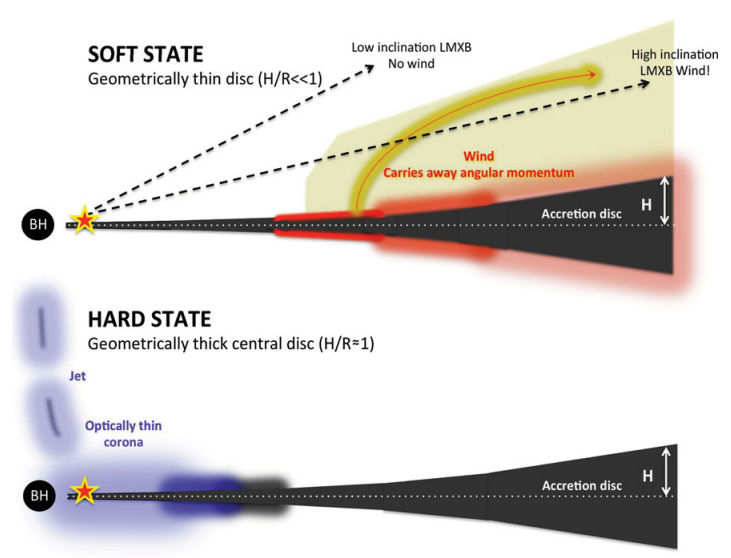
\includegraphics[width=1.0\textwidth]{figures/01-intro/ponti_wind_cartoon.png}
\caption
{
{\sl Credit: Ponti et al. 2012}. 
A cartoon illustrating the expected geometry of soft-state LMXB winds.
} 
\label{fig:ponti_hid}
\end{figure}


\subsection{AGN and Quasars}
\label{sec:agn_winds}

\subsubsection{Broad Absorption Line Quasars}

\subsubsection{Warm Absorbers}

\subsubsection{Ultra-fast Outflows}


\begin{figure}
\centering
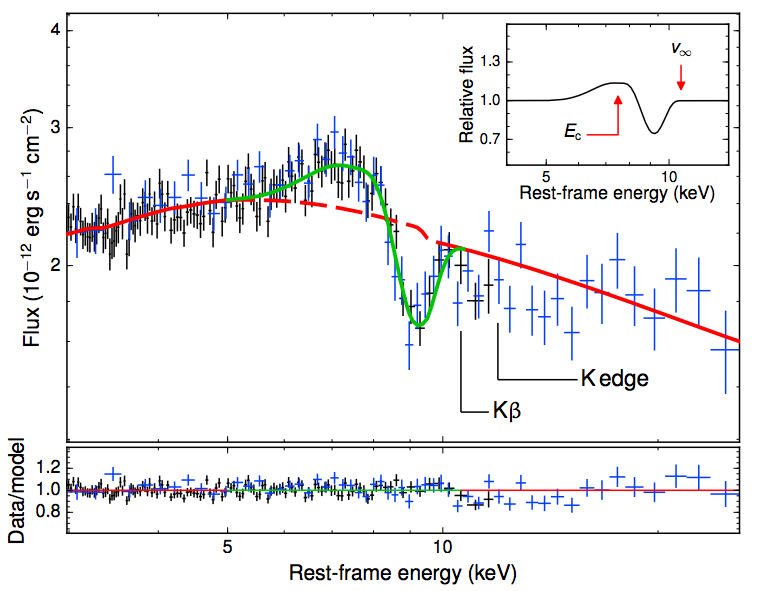
\includegraphics[width=1.0\textwidth]{figures/02-outflows/nardini_pds456.png}
\caption
{
{\sl Credit: Nardini et al. 2015}. 
X-ray spectrum fitted with a P-Cygni profile from a spherical outflow model.
{\sl XMM-Newton} data is shown in black with two combinaed {\sl NuStar}
observations in blue.
} 
\label{fig:nardini}
\end{figure}


\subsection{Stellar Winds}

Although stellar winds are clearly not accretion disc winds,
they provide a useful, and better understood, testing ground for much
of the physics of radiatively-driven outflows.

\subsubsection{Clumping}




\section{Driving Mechanisms}

Let us consider a parcel of ideal gas. By imposing nothing more than
conservation of mass, energy and momentum on that parcel we can write down
three equations of hydrodynamics
\footnote{I stress that these equations are not used in hydrodynamic
simulations in this thesis (see section ?, for example); 
they are discussed here because they provide a natural reference point
for exploring potential driving mechanisms for winds in accreting systems.
}

\begin{equation}
\label{eq:continuity}
\frac{D \rho}{Dt} + \rho \nabla \cdot \vec{v} = 0
\end{equation}

\begin{equation}
\label{eq:motion}
\rho \frac{Dv}{Dt} = -\nabla P + \frac{1}{4 \pi}(\nabla \times \vec{B}) \times \vec{B} + \rho \vec{F}_{rad} + \rho \vec{g}
\end{equation}

\begin{equation}
\label{eq:energy}
\rho \frac{D}{Dt} \left(\frac{e}{\rho}\right) = P \nabla \cdot \vec{v} + \rho \cal{L}
\end{equation}

Here $D$ denotes a derivative within the comoving frame of the gas parcel, $\vec{v}$ is the velocity,
$\rho$ is the gas density, $\vec{B}$ is the local magnetic field, $\vec{F}_{rad}$ is the radiation
force per unit mass and $\vec{g}$ denotes the gravitational acceleration vector.
Equation~\ref{eq:continuity} is the {\em continuity equation} and describes conservation of mass. 
Equation~\ref{eq:motion} is the {\em equation of motion} and describes conservation of momentum.
Equation~\ref{eq:energy} is the {\em equation of energy conservation}. 
We can use equation~\ref{eq:motion} to neatly demonstrate how an outflow can be driven. I have 
deliberately written the equation so that all the force terms lie on the RHS. We can then see that
for an outflow to be driven from an accreting object one simply needs one of the terms on
the RHS to dominate over gravity, $\rho \vec{g}$. These terms thus signify three potential
driving mechanisms.

\begin{itemize}
	\item Magnetic Forces, $\frac{1}{4 \pi}(\nabla \times \vec{B}) \times \vec{B}$.
	\item Radiative Forces, $\rho \vec{F}_{rad}$.
	\item Thermal Pressure, $-\nabla P$.
\end{itemize}

We can now examine under what physical conditions (and in which corresponding astrophysical objects)
we might expect these forces to overcome gravity and cause a parcel of mass to escape to infinity.
In other words: {\em what might drive a wind?}

\subsection{Thermal Winds}

In hydrostatic equilibrium (HSE), thermal pressure balances gravity and no other forces 
are present, meaning that the equation of motion can be written as 
\begin{equation}
\label{eq:hse}
\rho \frac{Dv}{Dt} = -\nabla P +  \rho \vec{g} = 0
\end{equation}
Clearly, if the thermal pressure is then significantly 
increased then this equilibrium condition no longer holds. 
This can occur in accretion discs at temperatures in excess of $\sim10^7$~K --
where other forces are negligible compared to thermal pressure -- 
and where the escape velocities are relatively low (i.e. far out in the disc).
Due to the temperature and gravity scalings, this means
that XRBs are natural candidates for showing evidence of thermally driven
winds. The outer disc can be heated to the Compton temperature by the central X-ray source,
potentially driving relatively high mass-loss rate outflows \citep{begelman1983,woods1996}. 
This driving mechanism has been proposed as a natural explanation
for the ever-present equatorial outflows in soft state XRBs \citep{ponti2012}.
However, they are much less likely candidates in CVs and AGN {\bf Discuss scaling
arguments with equations?}.


\subsection{Radiatively Driven Winds}
\label{sec:rad_winds}

\subsection{Line-driven Winds}

\subsection{Magneto-centrifugal Winds}

\section{Accretion Disc Wind Models}


\section{A Kinematic Prescription}




\section{The really, really big picture: AGN Feedback}

The event horizon of a $10^9~M_\odot$ BH is approximately 
$10^{15}$~cm, a billionth of the size of a typical galactic bulge. This is 
roughly the difference in size between a small coin and the radius of the 
Earth. Despite this vast different in scale, there are multiple
pieces of evidence that the physics on the scale of the gravitational
radius of the BH really does affect the evolution and dynamics of its host galaxy.
I shall briefly discuss the evidence for this statement, and 
assess the potential role of winds together with alternative mechanisms.

\subsection{Observational evidence for feedback}

Perhaps the most famous pieces of evidence for some kind of long-distance 
relationship between a central BH and its host galaxy are the 
$M_{BH}-\sigma_*$ and $M_{BH}-M_{bulge}$ correlations, shown in figures~\ref{fig:msigma}
and \ref{fig:mbulge} respectively.

\nocite{mcconnell2013,gultekin2009}
\begin{figure}
\centering
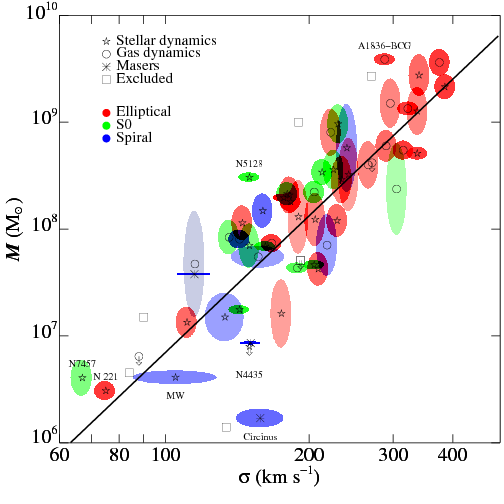
\includegraphics[width=0.7\textwidth]{figures/02-outflows/msigma.png}
\caption
{
{\sl Credit: Gultekin et al. 2009}. 
The $M_{BH}-\sigma_*$ correlation.
} 
\label{fig:mbulge}
\end{figure}

\begin{figure}
\centering
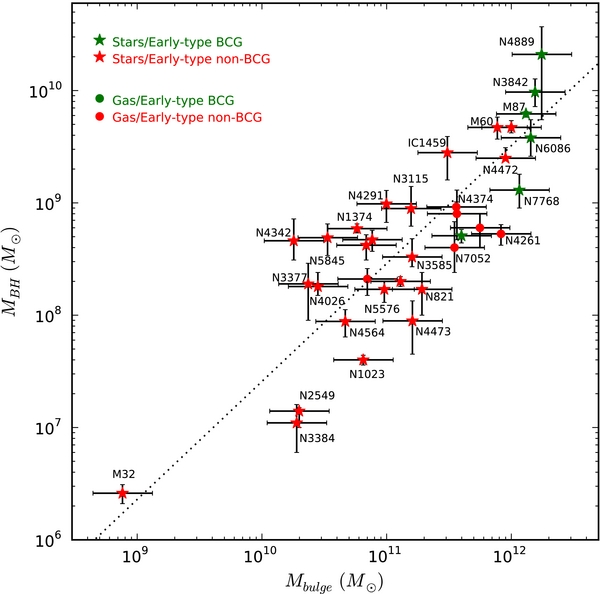
\includegraphics[width=0.7\textwidth]{figures/02-outflows/mbulge.jpg}
\caption
{
{\sl Credit: McConell \& Ma 2013}. 
The $M_{BH}-M_{bulge}$ correlation.
} 
\label{fig:mbulge}
\end{figure}

\subsection{Radiative or quasar mode feedback}

\subsection{Kinetic or radio mode feedback}

\subsection{In-situ Explanations}


